\documentclass{article}

\usepackage[margin=0.5in]{geometry}
%\geometry{legalpaper, landscape, margin=1in}

\usepackage{graphicx} % Required for inserting images

\usepackage{biblatex} %Imports biblatex package
\addbibresource{citations.bib} %Import the bibliography file

\usepackage{amsmath}
\usepackage{amsfonts}
% for code formatting:
\usepackage{listings}
%\lstset{
%  basicstyle=\ttfamily,
%  columns=fullflexible,
%  frame=single,
%  breaklines=true,
%  postbreak=\mbox{\textcolor{red}{$\hookrightarrow$}\space},
%}

\usepackage{textcomp}

\title{First Milestone -  Tools and Techniques}
\author{Kenneth L  Meyer, Jenil Shah, Rodrigo Gonzalez}
\date{October 19th, 2023}

\begin{document}

\maketitle

%\section{Introduction}

%task list:
%\begin{enumerate}
%    \item \textbf{Kenneth/Jenil} Governing equations, nomenclature, computational domain, and boundary conditions.
%    \item \textbf{Rodrigo} Expressions for a manufactured analytical solution and corresponding right hand side q and boundary conditions Tb, for both the 2D and 3D cases.
%    \item Numerical Method:
%    \begin{enumerate}
%        \item \textbf{Jenil} Provide 2nd- and 4th-order (central) finite-difference approximations for the second derivative in the heat equation. Make sure to include the leading order of the truncation error. Provide discrete approximations of the heat equation using these formulations (again including truncation error).
%        \item \textbf{Jenil} Provide representative figures of 1D and 2D discretized grids indicating domain size, grid sizes (including variable names that will be referenced in your input file later on), and finite-difference notation for neighboring cells. Be sure to indicate whether your scheme is node-based or cell-based.
%        \item \textbf{Rodrigo} Outline the linear system that you will form as part of the numerical method. Indicate the number of non-zero entries on an interior row of the matrix for the 1D, and 2D cases with both finite difference schemes (bonus points will be given for nice figures which highlight the structure of the resulting matrices).
%        \item \textbf{Kenneth} In pseudo-code, provide a simple iterative solution mechanism for the resulting linear system using: i. Jacobi ii. Gauss-Seidel
%        \item \textbf{Kenneth} Estimate the amount of memory required (using double-precision) to implement your numerical methods. Recall that the system matrix is sparse, and that you do not need to store the zero entries of the matrix.
%        \item \textbf{everyone} You may add bibliographic references as needed.

%    \end{enumerate}

%\end{enumerate}

\section{Governing equations, nomenclature, etc}

The goal of this project is to use finite-difference schemes to solve the heat equation in 1D and 2D space. In 1D, we are solving

$$
\begin{cases}
    -k \frac{d^2}{dx^2}T(x) = q(x) \text{ in } \Omega \\
    T(x) = T_b(x) \text{ on } \partial\Omega \\
\end{cases} 
$$

and in 2D,

$$
\begin{cases}
    -k \nabla^2 T(x,y) = q(x,y) \text{ in } \Omega \\
    T(x,y) = T_b(x,y) \text{ on } \partial\Omega
\end{cases} 
$$

where $\Omega = [0,1]^d$ is the physical and computational domain in both cases. The coefficient $k$ is a constant and as shown above, the boundary conditions are Dirichlet conditions.

\subsection{Manufactured solution: 1D case.}
Let the manufactured solution be: 

\begin{equation*}
    T(x) = \text{sin}(2 \pi x)
\end{equation*}

Then it solves the following equation

$$
\begin{cases}
    -k \frac{d^2}{dx^2}T(x) = \text{sin}(2\pi x) =: q(x)\text{ in } \Omega \\
    T(x) = 0 \text{ on } \partial\Omega \\
    k = 1/(4\pi^2)
\end{cases} 
$$

\subsection{Manufactured solution: 2D case.}
Let the manufactured solution be: 

\begin{equation*}
    T(x,y) = \text{sin}(2 \pi x)\text{ sin}(2 \pi y)
\end{equation*}

Then it solves the following equation

$$
\begin{cases}
    -k \nabla^2 T(x,y) = \text{sin}(2 \pi x)\text{ sin}(2 \pi y) =: q(x,y)\text{ in } \Omega \\
    T(x,y) = 0 \text{ on } \partial\Omega \\
    k = 1/(8\pi^2)
\end{cases} 
$$

These two manufactured solutions will serve to quantify the error produced by the numerical scheme by comparing approximated and the analytical solutions of these two problems. 
%--------------------------------------
\section{Numerical Methods}
\subsection{Finite Difference approximations}
\subsubsection{2$^{nd}$ order approximation}
1D case:
\begin{equation}
\begin{split}
    \frac{T(x+\Delta x) - 2T(x) + T(x-\Delta x)}{\Delta x^2}
    +\mathcal{O}(\Delta x^2)= -\frac{q(x)}{k}
\end{split}
\end{equation}
2D case:
\begin{equation}
\begin{split}
    \frac{T(x+\Delta x, y) - 2T(x,y) + T(x-\Delta x, y)}{\Delta x^2} & +\frac{T(x, y+\Delta y) - 2T(x,y) + T(x, y-\Delta y)}{\Delta y^2} \\
    & +\mathcal{O}(\Delta x^2)= -\frac{q(x)}{k}
\end{split}
\end{equation}

\subsubsection{4$^{th}$ order approximation}

1D case:
\begin{equation}
    \begin{split}
    &\frac{-T(x+2\Delta x) + 16T(x+\Delta x) -30T(x) +16T(x-\Delta x) -T(x-2\Delta x)}{12\Delta x^2}\\
    & +\mathcal{O}(\Delta x^4) = -\frac{q(x)}{k} 
\end{split} 
\end{equation}

2D case:
\begin{equation}
    \begin{split}
    &\frac{-T(x+2\Delta x, y) + 16T(x+\Delta x, y) -30T(x,y) +16T(x-\Delta x, y) -T(x-2\Delta x, y)}{12\Delta x^2} \\
    &+\frac{-T(x, y+2\Delta y) + 16T(x, y+\Delta y) -30T(x,y) +16T(x, y-\Delta y) -T(x, y-2\Delta y)}{12\Delta y^2}\\
    & +\mathcal{O}(\Delta x^4) = -\frac{q(x)}{k} 
\end{split}
\end{equation}

The truncation error in the central second order approximation are $\mathcal{O}(h^2)$, whereas in the fourth order approximation, they go as $\mathcal{O}(h^4)$ (where h is max($\Delta y, \Delta x$), W.L.G, we assume it is $\Delta x$)
The above equations are taken from the linked PDF\footnote{https://www.mech.kth.se/~ardeshir/courses/literature/fd.pdf}.
\subsection{Representative Figures$^{\ref{fig:finite_diff_fig1} \ref{fig:finite_diff_fig2}}$}
\begin{figure}
    \centering
    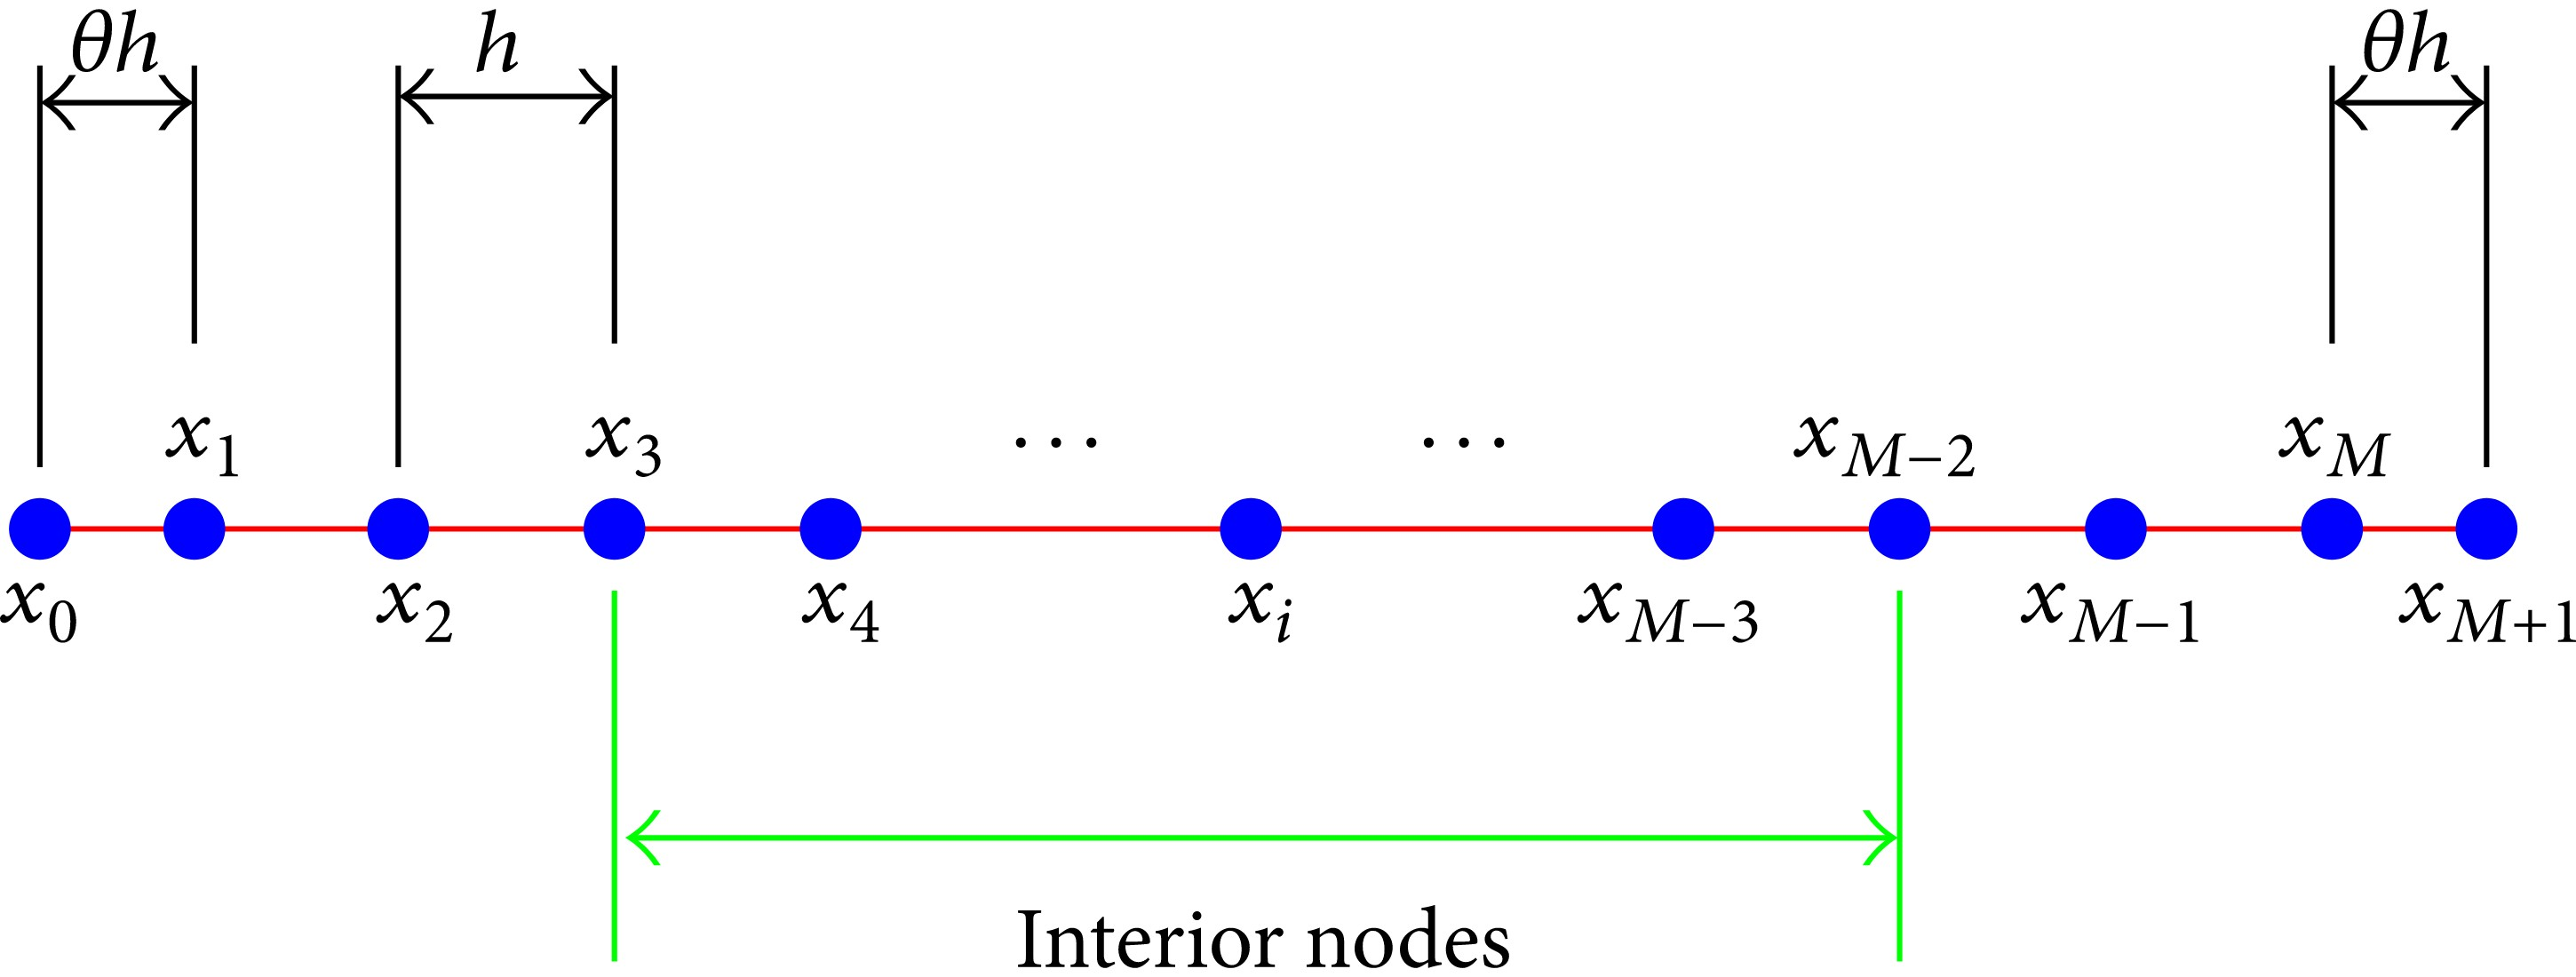
\includegraphics[width=0.4\columnwidth]{Figures/1Dheateqn.jpg}
    \caption{1D difference representative figure}
    \label{fig:finite_diff_fig1}
\end{figure}
\begin{figure}
\centering
    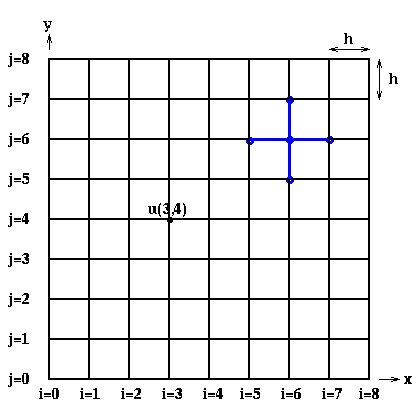
\includegraphics[width=0.4\columnwidth]{Figures/2DHeat2.png}
    \caption{2D Finite difference representative figure}
    \label{fig:finite_diff_fig2}
\end{figure}

Figure \ref{fig:finite_diff_fig1} \footnote{https://www.hindawi.com/journals/ana/2016/8376061/fig1/} represents the 1D and Figure \ref{fig:finite_diff_fig2} \footnote{http://people.eecs.berkeley.edu/~demmel/cs267/lecture17/lecture17.html} represents the 2D system. Our interval width is h, and i and j are our choices for the counters in x and y direction respectively. Our system is node-based.

\subsection{Linear Systems}
\subsubsection{Second Order, 1D case}
Let 

\begin{equation*}
\Vec{\alpha} = 
     \begin{bmatrix}
        T_1 \\
        \vdots \\
        T_{N-1} 
    \end{bmatrix}  
\end{equation*}

where $T_i = T(x_i)$ corresponds to the approximated value of $T$ - the unknown - at the point $x_i$ where $x_i = i*h$, and $h = 1/N$ (or $\delta x = \delta y$ to match the previous' section notation) and $N$ is the number of sample points in the domain. Our goal is to find $\Vec{\alpha}$.

To do this, we approximate the second derivative with a second order finite difference formula in the previous section to obtain

\begin{equation*}
-(k/h^2) (T_{i-1} -2 T_i + T_{i+1}) = q(x_i)
\end{equation*}

Repeating this for $i = 1 \ldots N-1$ leads to $N-1$ independent equations that can be vectorized in the following linear system

\begin{equation*}
\mathbf{M_2} \Vec{\alpha} = \Vec{q}
\end{equation*}

where 

\begin{equation*}
    \mathbf{M_2}  = -(k/h^2)\text{ tridiag}(1, -2 , 1)
\end{equation*}

That is, $\mathbf{M_2}$ is the matrix that contains a $-2$ on the diagonal, and $1$ on the first upper and sub diagonal. Moreover, we define

\begin{equation*}
\Vec{q} = 
     \begin{bmatrix}
        q_1 \\
        \vdots \\
        q_{N-1}
    \end{bmatrix}  
\end{equation*}

where $q_i = q(x_i)$. Note that in this case each row of the matrix has $N-1$ entries, but on the interior of the matrix only $3$ are non-zero.

\subsubsection{Fourth Order, 1D case}

Allowing $\Vec{\alpha}$ and $\Vec{q}$ to be defined as before, we arrive at a similar system. However, in this case we have 

\begin{equation*}
    \mathbf{M_4} = -(k/12 h^2)\text{ sixdiag}(-1, 16, -30, 16, -1)
\end{equation*}

Therefore, in each interior row there are only $6$ non-zero entries.

\subsubsection{Second Order, 2D case}

Let 

\begin{equation*}
\Vec{\alpha_i} = 
     \begin{bmatrix}
        T(x_i,y_1) \\
        \vdots \\
        T(x_i, y_{N-1}) 
    \end{bmatrix}  
\end{equation*}

As before, we let $x_i = y_i = ih$ with $h = 1/N$ and $N$ is the number of sample points in the domain. These is a vector containing all the $y$ points associated with the $x_i$ point in the domain. Then, applying the finite difference formula, we obtain

\begin{equation*}
\big( \frac{1}{h^2} \begin{bmatrix}
\mathbf{I} & -2\mathbf{I} & \mathbf{I}
\end{bmatrix} + \big(\begin{bmatrix}
\mathbf{0} & \mathbf{M_2} & \mathbf{0} 
\end{bmatrix} \big) \begin{bmatrix}
\Vec{\alpha}_{i-1} \\
\Vec{\alpha}_i \\
\Vec{\alpha}_{i+1}
\end{bmatrix}  = \Vec{q}_i
\end{equation*}

Where $\mathbf{I}$ is the $(N-1)$ identity matrix, $\mathbf{M_2}$ is defined as before, and 

\begin{equation*}
\Vec{q}_i = 
     \begin{bmatrix}
        q(x_i,y_1) \\
        \vdots \\
        q(x_i, y_{N-1}) 
    \end{bmatrix}  
\end{equation*}

Repeating for each $i = 1, \ldots, N_1$ we get a system that can be conveniently written with Kronecker products as follows:

\begin{equation*}
\big( \mathbf{M_2} \otimes \mathbf{I} +  \mathbf{I} \otimes \mathbf{M_2} \big) \Vec{\alpha} = \Vec{q}
\end{equation*}

where we solve for 

\begin{equation*}
\Vec{\alpha} = 
     \begin{bmatrix}
        \Vec{\alpha}_1 \\
        \vdots \\
        \Vec{\alpha}_{N-1}
    \end{bmatrix}  
\end{equation*}

and $\Vec{q}$ is defined in a similar fashion. 

\subsubsection{Fourth Order, 2D case}

Allowing $\Vec{\alpha}$ and $\Vec{q}$ to be defined as before, we arrive at a similar system. However, in this case we use $M_4$. In other words, we solve

\begin{equation*}
\big( \mathbf{M_4} \otimes \mathbf{I} +  \mathbf{I} \otimes \mathbf{M_4} \big) \Vec{\alpha} = \Vec{q}
\end{equation*}

\subsection{Iterative Solution Mechanisms}
%The resulting linear system that will be formed can be solved by simple iterative solution mechanisms. The two methods that will be used in this project will be the Jacobi method and Gauss-Seidel. Note that for both guesses, the initial guess a \texttt{x\_0} i.e. $x^{(0)}$, can be set to the zero vector.

\subsubsection{Jacobi Method}

% OG Jacobi, without sparsity
The jacobi method can be used to solve a general linear system $Ax=b$ where $A \in \mathbb{R}^n$ is our coefficient matrix, $b \in \mathbb{R}$, and $x \in \mathbb{R}^n$ is our vector of unknowns. With our linear system, $\mathbf{M} \Vec{\alpha} = \Vec{q}$, these correspond to $A, x, \text{ and } b$. We will use an initial guess or the 0 vector for \texttt{x\_0} i.e. $x^{(0)}$ in both Jacobi and Gauss-Seidel (in the next section)

The jacobi method assumes that the system has a unique solution and that $A$ has no zeros on its main diagonal; $a_{ii} \neq 0 \: \forall \: i = 1, .., n$.


$$
    x_{k+1} = D^{-1}(E + F)*x_k + D^{-1}*b
$$

is the jacobi method in vector form \cite{saad03:IMS}.
% note: we don't need to use the matrix method; we'll be storing things sparsely anyways.

A sample implementation of the Jacobi Method, in psuedocode, is shown below:

\begin{lstlisting}[caption={Jacobi Method Psuedocode \cite{saad03:IMS}},captionpos=b,escapeinside={(*}{*)}]
    Given: A, b, tolerance tol, and max its N, and initial guess x_0
    x_k = x_0
    k = 1
    while (*(k $\leq$ N)*)
        x_k_1 = (*$D^{-1}$*)(E + F)x_k + (*$D^{-1}$*)b
        if ||x_k_1 - x_k|| < tol
            break
        x_k = x_k_1
    return x_k_1
\end{lstlisting}

%where $D, E, $ and $F$ are defined from the following image:

%\begin{figure}
%    \centering
%    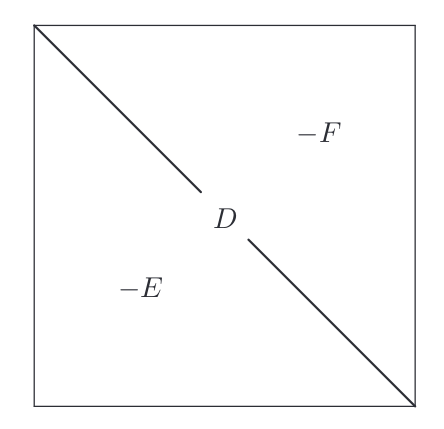
\includegraphics[height=0.15\textheight]{Figures/jacobi_matrix_partitioning.png} 
%    \caption{Iterative method matrix structure \cite{saad03:IMS}}
%    \label{fig:DEF_matrix_structure}
%\end{figure}

where $D$ is the diagonal of $A$, and $-E$ and $-F$ are its strictly lower and upper diagonals, respectively.

%Note that to exploit sparsity, it may be easier to use a component-wise form of the Jacobi Method defined by:

%$$
%    \zeta_i^{(k+1)} = \frac{1}{a_{ii}}(\beta_i - \sum_{j=1, j \neq i}^n a_{ij}\zeta_j^{(k)}); i = 1, ... ,n
%$$

%which is equivalent to the equation presented in the psuedocode, 


% try to find a good way to include the pseudocode; this is not perfect here.
% need to:
% 1. check stopping criterion
% 2. find a textbook that's better than the notes I found online
%if (*$||\textbf{x} - X)|| < \texttt{tol}$*)
%\begin{lstlisting}[escapeinside={(*}{*)}]
%    (*$A = [a_{ij}], \textbf{b}, \textbf{X0} = \textbf{x}^{(0)}$*) tolerance % (*\texttt{tol}*), and max its (*$N$*),
%\end{lstlisting}


% comment on how sparsity can be exploited to speed up computation time.

\subsubsection{Gauss-Seidel}

Gauss-Seidel is a similar iterative solution scheme. However, it updates the approximate solution immediately after the new component is determined. % idrk what this means, I don't think the refence I used explains it well.

The vector form of the Gauss-Seidel method is
$$
    x_{k+1} = (D - E)^{-1}Fx_k + (D-E)^{-1}b
$$
and pseudocode for the Gauss-Seidel method is found below:

\begin{lstlisting}[caption={Gauss-Seidel Psuedocode \cite{saad03:IMS}},captionpos=b, escapeinside={(*}{*)}]
    Given: A, b, tolerance tol, and max its N, and initial guess x_0
    x_k = x_0
    k = 1
    while (*(k $\leq$ N)*)
        x_k_1 = (*$(D - E)^{-1}$*)F*x_k + (*$(D-E)^{-1}$*)*b
        if ||x_k_1 - x_k|| < tol
            break
        x_k = x_k_1
    return x_k_1
\end{lstlisting}

Note that * denotes matrix-vector multiplication.

%and similarly to the Jacobi method, the component-wise form of the Gauss-Seidel method is
%$$
%    \zeta_i^{(k+1)} = \frac{1}{a_{ii}}( -\sum_{j=1}^{i-1} a_{ij}\zeta_j^{(k+1)} -\sum_{j=i+1}^n a_{ij}\zeta_j^{(k)} + \beta_i); i = 1, ... ,n
%$$

%which could potentially be useful \cite{saad03:IMS}.

\subsection{Memory Requirements}

If our matrices were dense, both Jacobi and Gauss-Seidel would have memory requirements of $\mathcal{O}(n^2)$ as $A \in \mathbb{R}^{nxn}$. However, the matrices derived from the finite-difference schemes will be sparse in nature. For the Jacobi Method, $\mathcal{O}(nm + 3n)$ memory will be used ($nm$ is the storage of $D^{-1},E,F$ matrices, and $3n$ to store $x^{(k)}$, $x^{(k+1)}$, and $b$). For Gauss-Seidel, $\mathcal{O}(\frac{1}{2}n^2 + \frac{1}{2}mn + 3n)$ memory will be used to store $(D-E)^{-1}, F, \text{ and } x^{(k)}, x^{(k+1)}, \text{ and } b$ respectively. Note that $m$ is the maximum number of non-zero entries in a row of $A$, and a sparse structure is lost when computing $(D-E)^{-1}$.

%If our matrices were dense, both Jacobi and Gauss-Seidel would have memory requirements of $\mathcal{O}(n^2)$ as $A \in \mathcal{R}^{nxn}$. However, the matrices derived from the finite-difference schemes will be sparse in nature. The matrix $A$ can be stored with memory of $\sim nm$, where $m$ is the number of non-zero diagonals in the matrix $A$, which depends on the finite difference method used and space (1D or 2D) of the problem. We will also have to store $x^{(k)}$, $x^{(k+1)}$, and $b$, so the memory requirements of the Jacobi Method will be $\mathcal{O}(n(m+3))$

%For Gauss-Seidel, there is a difference in the matrix being inverted. $D^{-1}$, which is computed in the Jacobi Method, is still a diagonal matrix, so no extra storage is needed. In Gauss-Seidel, $(D - E)^{-1}$ is computed, and this does not necessarily preserve a sparse structure. Thus, this quantity dominates memory storage requirements, and the Gauss-Seidel method requires ~$\mathcal{O}(\frac{1}{2}n^2)$ memory.

%Note that both of these calculations were done for the iterative solution schemes in matrix form.
%--------------------------------------

%\bibliographystyle{plain}
%\bibliography{citations.bib}
\printbibliography %Prints bibliography

\end{document}
